%%=============================================================================
%% Inleiding
%%=============================================================================

\chapter{\IfLanguageName{dutch}{Inleiding}{Introduction}}
\label{ch:inleiding}

\section{\IfLanguageName{dutch}{Context}{Context}}
\label{sec:context}

Webapplicaties die data verwerken hebben nood aan een apart systeem die de data op aanvraag van de webapplicatie in kwestie kan voorzien. De software die de communicatie tussen beide systemen voorziet is architecturaal zo gebouwd om goed te werken op het Web doordat de data-uitwisseling gebeurt via het internet. \\
Dergelijke systemen kunnen “RESTful web services” genoemd worden, waar REST staat voor “Representational State Transfer”. Het impliceert een architectuur voor web-services waarbij een uniforme interface wordt gebruikt voor het bekomen van verbeteringen aan bepaalde eigenschappen, zoals performantie of schaalbaarheid. \\
De communicatie tussen de webapplicatie en web-service gebeurt via een \gls{HTTP}-protocol, wat typisch is voor \gls{REST}-architectuur. Het protocol volgt een klassiek model voor client/server-architectuur waarbij de client, zijnde de webapplicatie, een connectie opent naar de server voor een aanvraag en vervolgens wacht op een antwoord.

Gebruikelijk worden \gls{REST}ful web-services ontwikkeld in een programmeertaal die geschikt is voor het toepassingsgebied. In belang van het onderzoek worden web-services aanzien als alleenstaande en onafhankelijke services die in een ``cluster'' geplaatst kunnen worden voor het doel van microservices. \\
De meest welbekende en populaire programmeertalen voor het ontwikkelen van web-services zijn Java, Python, C\# en Node.js. De laatste van de opgenoemde vier is de jongste en lijkt daarmee het minst matuur. Niets is minder waar. Met de intentie om JavaScript, de alom bekende Web-taal, naar de backend te brengen heeft het de markt met stormenderhand veroverd.

\subsection{\IfLanguageName{dutch}{Wat is JavaScript?}{What is JavaScript?}}
\label{subsec:wat-is-javascript}

De scripttaal JavaScript werd gecreëerd door \emph{Brendan Eich} in 1995 gedurende zijn tijd als werknemer bij \emph{Netspace Communications}. Elke scripttaal is een programmeertaal in zijn eigen recht en buiten JavaScript zijn er ook nog anderen, waaronder bash, Ruby, Perl, Python, ... \\
In 1997 werd JavaScript een \gls{ECMA}-standaard en behoort nu tot één van de meest gebruikte programmeertalen voor het Web. JavaScript runt nu out-of-the-box in alle browsers waardoor het kan draaien op elk \gls{OS} en maakt dat JavaScript platform onafhankelijk is. Elke browser heeft zijn eigen omgeving die JavaScript interpreteert, zo heeft bijvoorbeeld \emph{Google Chrome} de V8 en \emph{Mozilla Firefox} SpiderMonkey.

Als programmeertaal kreeg JavaScript vooral veel aandacht als scripttaal voor het Web. Samen met \gls{HTML} en \gls{CSS} vormt het een ideale stack voor webapplicaties in elke browser. De \gls{HTML} zorgt voor de inhoudelijke structuur en \gls{CSS} definieert daarbij een verzameling aan regels die de inhoud stijlt. Aanvullende maakt JavaScript het mogelijk om de statische \gls{HTML} dynamisch te maken. Het aanpassen van de inhoud afhankelijk van gebruikersinteractie of het spelen van animaties wordt gebruikelijk gedaan door middel van JavaScript.

JavaScript wordt vooral gebruikt omwille van zijn simpliciteit, relatief eenvoudige leercurve, flexibiliteit en ontwikkellaarsvriendelijkheid. Het is geschreven voor een runtime-omgeving, wat concreet betekend dat de code in een omgeving moet uitgevoerd worden die de JavaScript interpreteert tijdens de uitvoering van de gehele applicatie. \\
Het uitvoeren van JavaScript gebeurd ``single-threaded''  en betekend dat de executie van JavaScript-functies telkens één per één verloopt. Dit zorgt ervoor dat er altijd enkel één functie wordt uitgevoerd per keer.

\subsubsection{\IfLanguageName{dutch}{ECMAScript}{ECMAScript}}
\label{subsubsec:ecmascript}

\gls{ECMA} is een organisatie die voor specifieke technologieën een standaard gaat opstellen. In 1997 werd voor algemeen bruikbare scripttalen een standaard opgesteld nadat JavaScript werd ingediend voor standaardisatie. De naam voor deze standaard is \gls{ECMA}-262. \\
\gls{ECMA}Script, of de meer vakjargon gebruikte term ES, is een scripttaal die geschreven is onder de \gls{ECMA}-262 standaard. JavaScript is een uitwerking van het \gls{ECMA}Script die de standaarden meer robuust maakt met het toevoegen van een wijd bruikbare \gls{API} bovenop de standaard.

\subsubsection{\IfLanguageName{dutch}{Single-threaded}{Single threaded}}
\label{subsubsec:single-threaded}

JavaScript is single-threaded binnen de omgeving dat het wordt uitgevoerd. Elke omgeving heeft zijn eigen interpretatie van de JavaScript, maar de code wordt synchroon afgehandeld, wat betekend dat elke lijn uitvoerbare code pas kan uitgevoerd worden wanneer de voorgaande volbracht is. De uitvoering wordt gefaciliteerd door gebruik te maken van één enkele ``call-stack'' en ``memory-heap'', vandaar \emph{single}-threaded. \\
De call-stack wordt constant gealloceerd in het geheugen en vormt in functie van JavaScript een verzameling van functies die uitgevoerd moeten worden. Zo weet de omgeving die de JavaScript interpreteert, zoals een browser, waar het zicht bevindt in de code. Bij het uitvoeren van de functies op de call-stack wordt het \gls{LIFO}-principe gehanteerd waarbij de laatste toevoeging op de stack als eerst wordt uitgevoerd. \\
Naast een stack voor het uitvoeren van bepaalde operaties is er ook een memory-heap. De heap wordt gebruikt voor het alloceren en vrijmaken van geheugen voor applicatie specifieke informatie in de vorm van variabelen. Een variabele kan allerlei soorten data bevatten, zoals een array, object of complexere datastructuren.

\begin{figure}[H]
    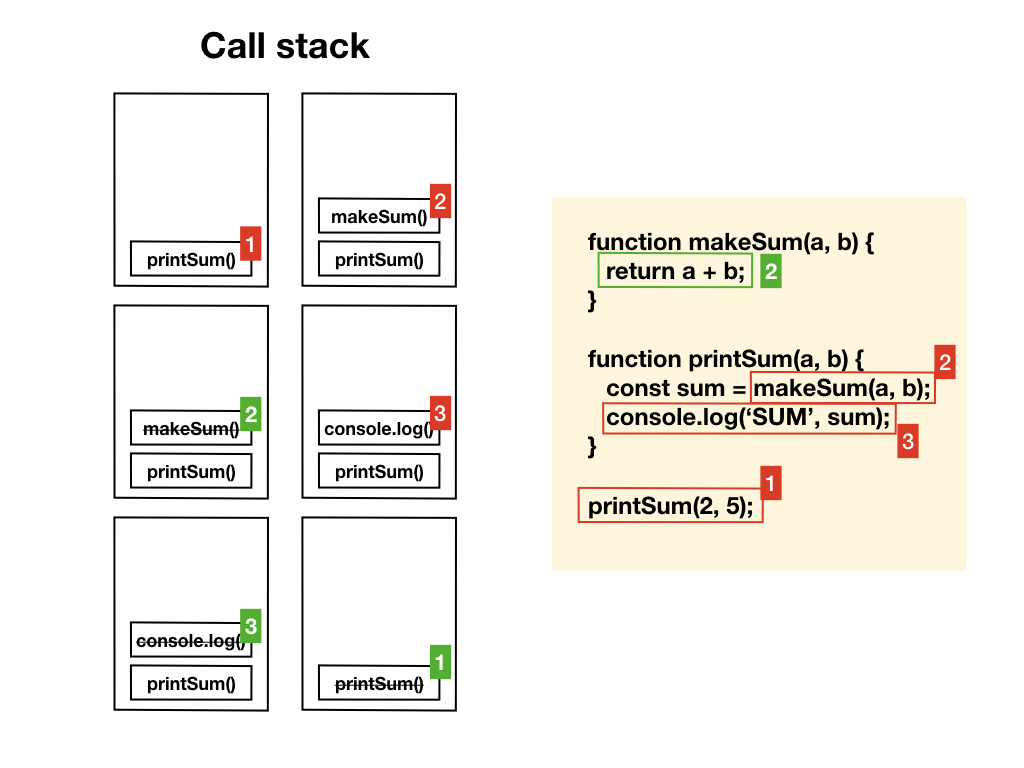
\includegraphics[width=\linewidth]{img/SingleThreaded.jpeg}
    \caption[Single threaded JS met call stack]{Single threaded uitvoering van JavaScript met behulp van call stack}
    \label{fig:single-threaded}
\end{figure}

\subsection{\IfLanguageName{dutch}{Backend JavaScript: Node.js}{Backend JavaScript: Node.js}}
\label{subsec:backend-javascript}

Met als uitgangspunt open-source te zijn, en te willen blijven, had Node.js niet de gegronde fundering en ondersteuning zoals andere backend-pioniers. Doorheen de jaren bouwde het een standvaste gemeenschap uit en kon daardoor een plek veroveren onder de groten in sprake van server-side ontwikkeling. \\
Dankzij de enorme groei en populariteit in gebruik ontstond er een globale opslagplaats voor fanatieke ontwikkelaars die hun creativiteit en \emph{skills} in Node.js wouden delen met de wereld. Deze opslagplaats werd voor het eerst beschikbaar in 2010 onder de naam \emph{NPM} of Node Package Manager. Nu is \gls{NPM} uitgegroeid tot het meest diverse en snelst groeiende ecosysteem voor JavaScript-libraries dat beschikbaar is.

Met het idee om JavaScript naar de backend te brengen werd Node.js voor het eerst uitgegeven in 2009 als open-source runtime-omgeving voor JavaScript. Node.js maakt het mogelijk voor ontwikkelaars om volledige webapplicaties te ontwikkelen in JavaScript voor zowel client- als server-side. Gebouwd op \emph{Google Chrome}'s V8-engine, en geschreven in C++, maakt het een JavaScript-vriendelijke omgeving met altijd toegang tot de nieuwste JavaScript-features. \\
Node.js biedt voor netwerken ingebouwde ondersteuning voor \gls{HTTP}-verzoeken. \gls{HTTP} is de meest populaire manier om data te versturen van de server naar een webpagina, en vice versa. Voor dataverwerking heeft Node.js native \gls{JSON}-serialisatie en -deserialisatie bij het versturen en ontvangen van \gls{HTTP}-verzoeken. \gls{JSON} is, samen met \gls{XML}, het meest voorkomende formaat voor het transporteren van data over \gls{HTTP} in moderne webapplicaties.

Node.js is een runtime-omgeving voor JavaScript en is gebouwd op \emph{Google Chrome}'s V8-engine. De uitvoering van JavaScript-code wordt geïnterpreteerd door V8's ``interpreter'', genaamd \emph{Ignition}, en omgezet naar machinetaal. De interpreter leest JavaScript-code op het moment van uitvoeren. Op hetzelfde moment wordt de code ook geanalyseerd voor mogelijke optimalisaties door V8's ``compiler'', genaamd \emph{TurboFan}. De technologie voor het interpreteren en compileren van JavaScript op het moment van uitvoeren heet \gls{JIT}-compilatie. De JavaScript wordt daarbij omgezet naar uitvoerbare machinetaal op het moment wanneer de code wordt uitgevoerd.

Als runtime-omgeving beschikt Node.js intern over toegang tot meerdere threads, ook wel een ``thread-pool'' genaamd, aangeboden door C++ waar Node.js in werd geschreven. De thread-pool biedt Node.js de mogelijkheid om JavaScript-code ook asynchroon uit te voeren door middel van ``callbacks'', wat in essentie JavaScript-functies zijn. \\
JavaScript is single-threaded en wordt synchroon uitgevoerd, zoals eerder aangegeven in sectie \ref{subsec:wat-is-javascrip}. De uitvoering van asynchrone code in een single-threaded omgeving creëert een blokkerende factor doordat de volledig thread geblokkeerd wordt door de asynchroon uit te voeren code. Om het blokkeren van de volledige thread te voorkomen bestaat er een software binnen de JavaScript runtime genaamd ``event loop'' voor het correct afhandelen van callbacks.

\subsubsection{\IfLanguageName{dutch}{Event loop}{Event loop}}
\label{subsubsec:event-loop}

De event loop is een software die bestaat binnen de JavaScript runtime-omgeving, waar het in verbinding staat met de call-stack en een ``callback-queue''. Terwijl de applicatie loopt gaat de event loop constant luisteren naar de callback-queue en call-stack. In figuur \ref{fig:event-loop} is te zien hoe de event loop is geplaatst tussen de twee binnen de runtime. \\
Vanaf het moment dat de call-stack leeg is neemt de event loop de eerste callback van de callback-queue en plaatst hem op de call-stack om uit te voeren. De callback-queue werkt volgens het \gls{FIFO}-principe waarbij de eerste callback op de callback-queue ook als eerste van de queue gehaald wordt.

\begin{figure}[H]
    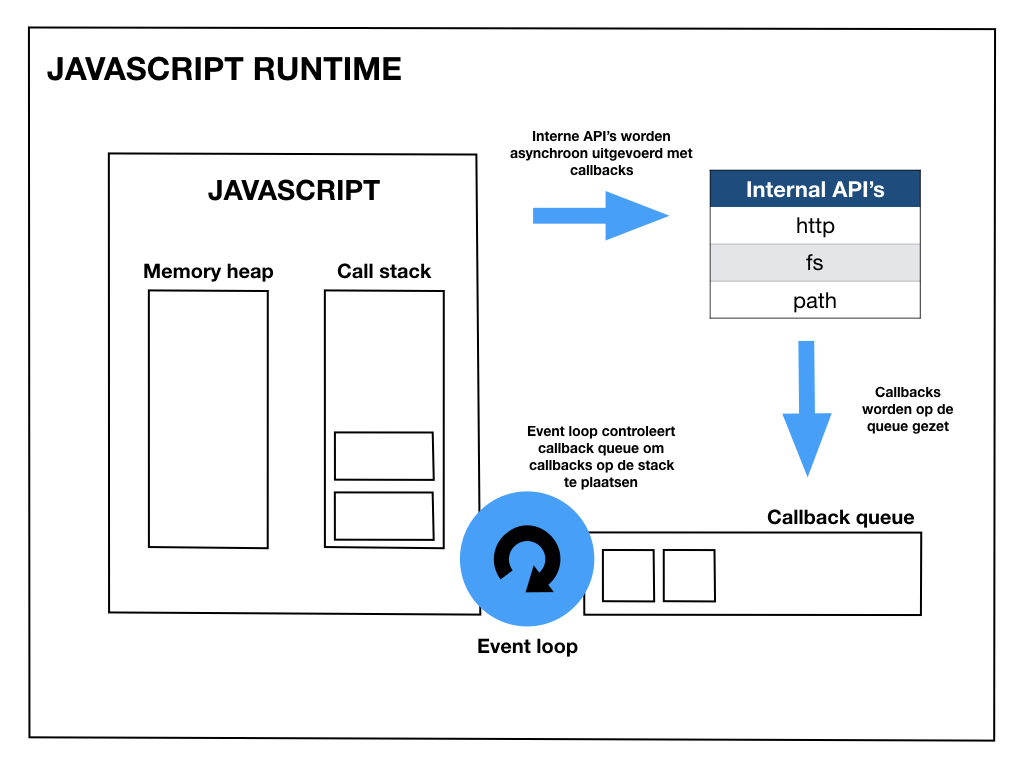
\includegraphics[width=\linewidth]{img/EventloopInRuntime.jpeg}
    \caption[Event loop in JS runtime]{Event loop binnen JavaScript runtime}
    \label{fig:event-loop}
\end{figure}

\subsubsection{\IfLanguageName{dutch}{Non-blocking I/O}{Non-blocking I/O}}
\label{subsubsec:non-blocking-io}

Niet-blokkerende I/O wijst op het uitvoeren van JavaScript-functies op een manier dat het niet de uitvoering van daarna komende blokkeert. Dit wordt in Node.js voorkomen door het asynchroon uitvoeren van de potentieel blokkerende JavaScript-functies door middel van callback-functies. De callbacks zorgen ervoor dat de asynchroon uit te voeren functies later nog mogelijke neveneffecten kunnen teweegbrengen. Executie van de applicatie kan op die manier voortgezet worden en kunnen er andere functies uitgevoerd worden, onafhankelijk van de asynchroon uitgevoerde functie. \\
Node.js heeft niet-blokkerende I/O, maar het is niet zo dat Node.js enkel niet-blokkerend is, het kan ook blokkerend zijn. Het blokkeren van de applicatie uitvoering wordt afgeraden door het single-threaded zijn van JavaScript.

\subsection{\IfLanguageName{dutch}{TypeScript}{TypeScript}}
\label{subsec:typescript}

JavaScript is een vrije en weinig expressieve programmeertaal. De code is dynamisch getypeerd waardoor de ontwikkelaar niet moet letten op typering van variabelen en functies die hij/zij aanmaakt. Overigens is JavaScript ook een ``zwakke'' programmeertaal, wat in essentie wilt zeggen dat de conversie naar een bepaald data type tijdens runtime niet wordt afgedwongen door de interpreter. Zo kan een variabele gedefinieerd worden als een string in samenstelling met een number, wat gezamenlijk impliciet getypeerd zal worden als een string.

TypeScript werd gecreëerd als taalveiligheid voor het vrije en dynamische JavaScript. Het werd geïntroduceerd in 2012 door \emph{Microsoft} en biedt een robuust type systeem aan dat als integratie over JavaScript optionele typering voorziet. Hierdoor wordt JavaScript niet meer dynamisch, maar wel statisch getypeerd. Het typeren is optioneel zodat elke TypeScript-file ook een correcte JavaScript-file blijft en zorgt ervoor dat een JavaScript-project incrementeel kan gemigreerd worden naar TypeScript. \\
De toevoeging van een type systeem maakt het mogelijk om statisch getypeerde JavaScript te schrijven, wat betekend dat de interpreter niet meer types tijdens runtime moet toekennen. TypeScript fungeert als compiler voor JavaScript en voegt een compile time toe vóór de runtime die de types gaat compileren vooraleer de applicatie wordt uitgevoerd. Met dat de interpreter geen types meer moet gaan toekennen tijdens runtime zorgt de compile time voor optimalisatie van de uit te voeren code.

De TypeScript compile time kan bij het compileren van de code fouten detecteren die niet opgevangen worden door de ontwikkelaar zelf of de editor. Bij het detecteren van fouten geeft TypeScript ``type-errors'' weer. Deze errors worden weergegeven in een ``stack trace'' die het volledige pad beschrijft van waar de error zich origineert. Sommige type-errors kunnen verwarrend en complex opgesteld zijn, waardoor de stack trace moeilijk te lezen en begrijpen is. \\
Het hele type systeem maakt het ontwikkelen van code binnen een TypeScript context veel uitgebreider. Zo kan JavaScript-code bestaande uit 5 lijnen omgezet naar TypeScript uitkomen op dubbel dat aantal, afhankelijk van wat getypeerd wordt. De types die telkens moeten toegevoegd worden om voordeel te halen uit het gebruik van TypeScript zorgen ervoor dat het ontwikkelingsproces langer duurt. Naast de meer uitgebreide code brengt TypeScript handige toevoegingen zoals automatische aanvulling van functies, functie-argumenten of properties en het automatisch importeren ervan.

Ondanks het extra ontwikkelwerk en eventuele complexiteit binnen de stack trace, heeft TypeScript een relatieve leercurve. De curve is afhankelijk van het niveau van de ontwikkelaar en zijn/haar eerdere ervaring met TypeScript of een andere getypeerde programmeertaal zoals Java. Toch blijken ontwikkelaars die compromis te willen maken. Onderzoek gevoerd door het team van \emph{State of JS}, in de vorm van een enquête bij 21.717 mensen, toont aan dat sinds 2016 de cijfers blijven stijgen voor ontwikkelaars die TypeScript leerde kennen, wouden gebruiken en daarna ook bleven gebruiken. Figuur \ref{fig:typescript-ervaring} toont een grafische voorstelling van de gebruikerservaringen met TypeScript van 2016 tot 2019.

\begin{figure}[H]
    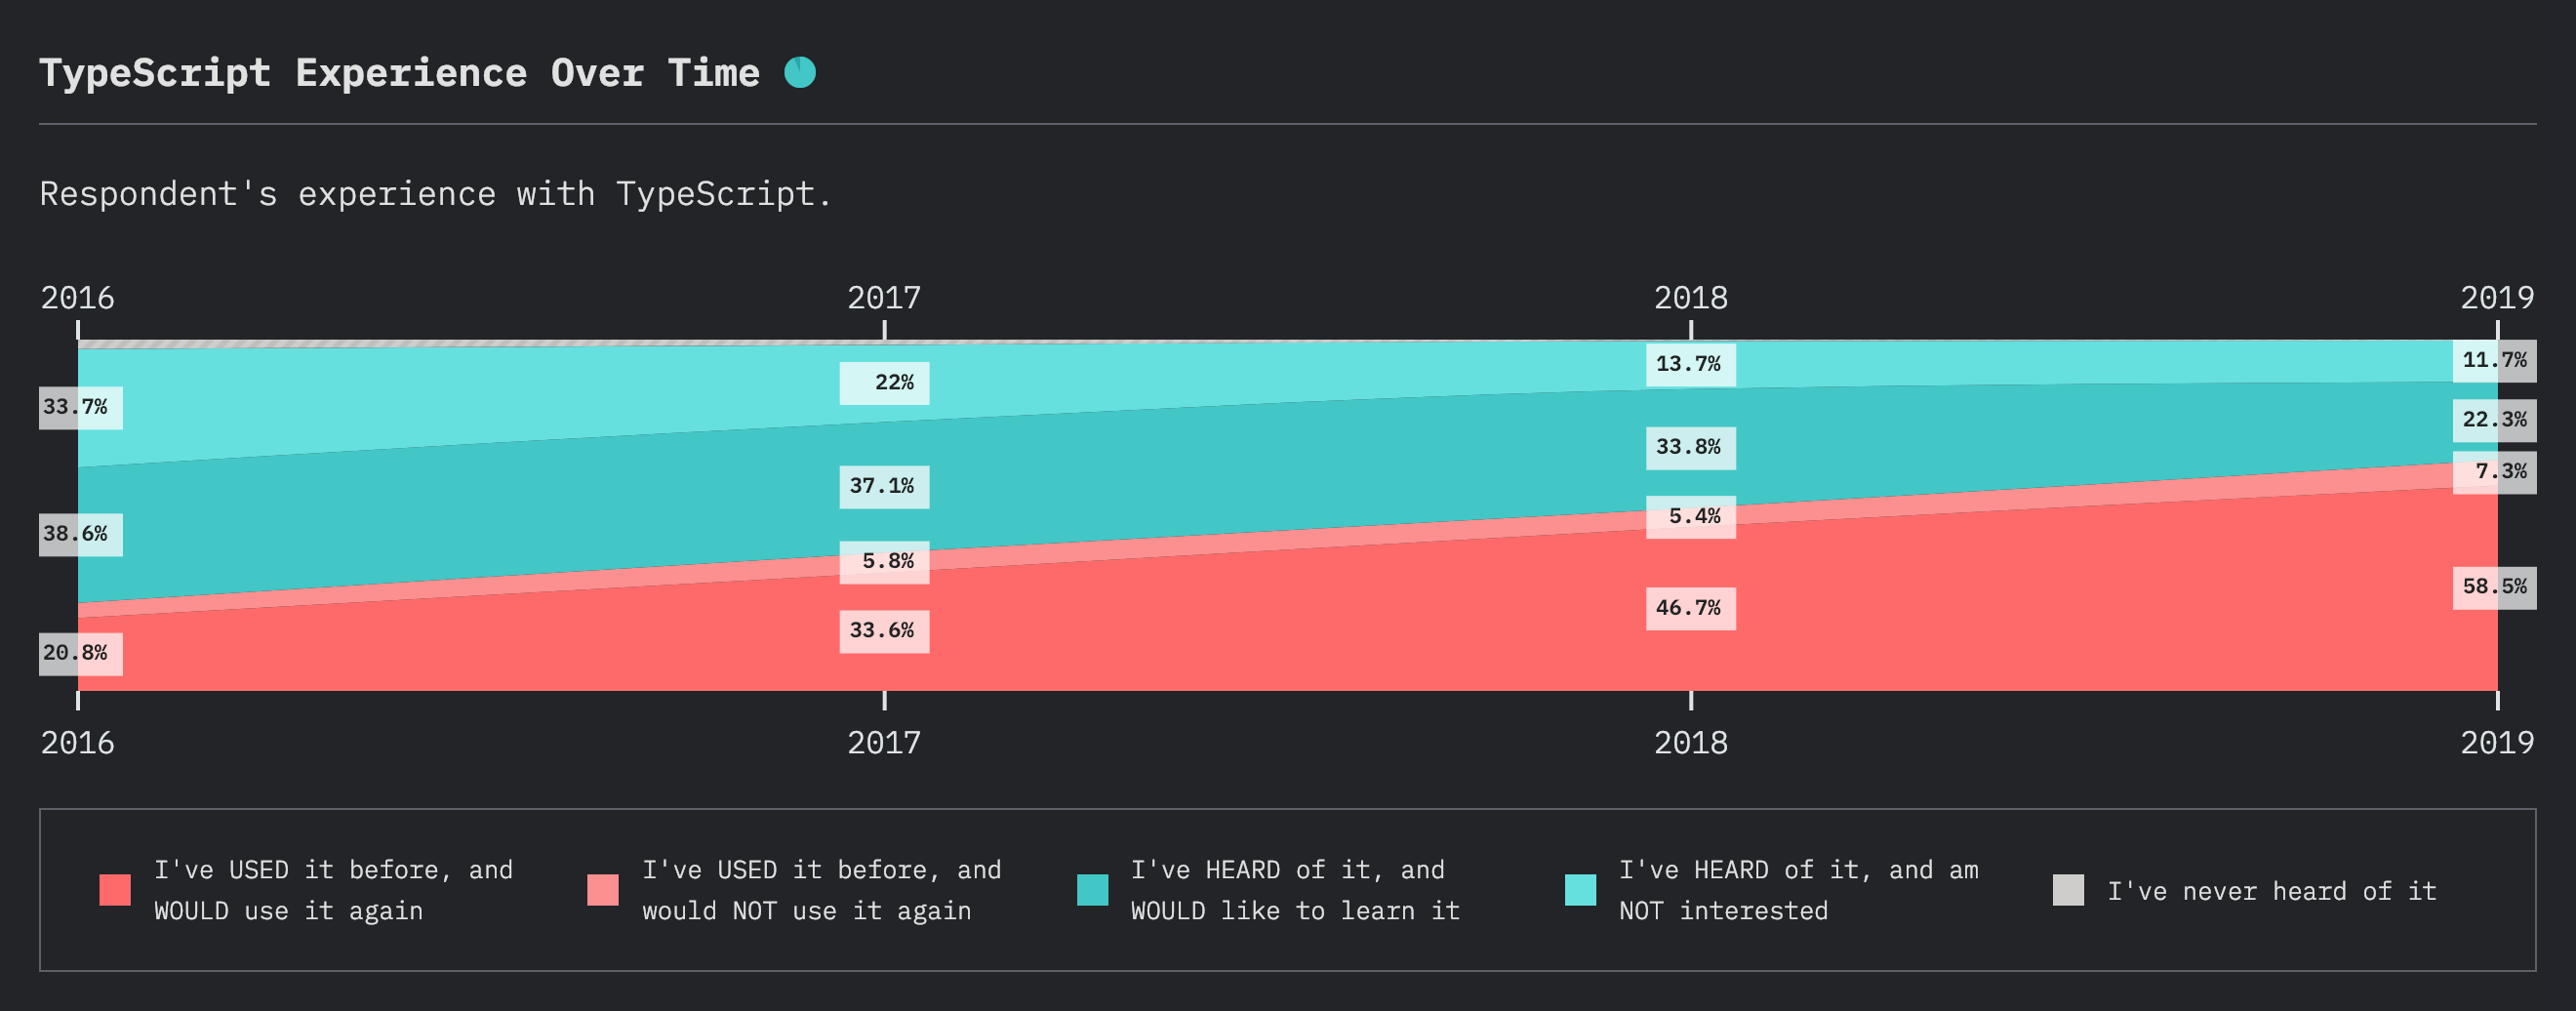
\includegraphics[width=\linewidth]{img/TypescriptExperience.png}
    \caption[Gebruikerservaringen met TypeScript]{Gebruikerservaringen met TypeScript van 2016 tot 2019}
    \label{fig:typescript-ervaring}
\end{figure}
% https://2019.stateofjs.com/javascript-flavors/typescript/

\subsection{\IfLanguageName{dutch}{Microservice-architectuur}{Microservice architecture}}
\label{subsec:microservice-architectuur}

Het eerste teken van microservices dook op in een presentatie van Peter Rodgers onder de naam ``Micro-Web-Services'', tijdens de \emph{Web Services Edge} conferentie in 2005. Later, op het einde van 2011, werd verder op de trend ingegaan en besloot een bestuur van software-architecten om de web-services van Micro-Web-Services, \emph{Microservices} te noemen. Deze architectuur werd dan de microservice-architectuur genaamd. \\
Een microservice wordt, in de letterlijke zin van het woord, beschouwd als een kleine service. Met klein wordt niet expliciet gezegd dat het een maximum bepaald aantal lijnen code mag omvatten, maar het is aanzienlijk kleiner dan de gebruikelijke monolieten die de volledige backend voorstellen van een business in één enkele web-service.

Een microservice-architectuur heeft als doel de benodigdheden van de business op te splitsen in kleine onafhankelijke services. Elke service heeft zijn eigen waarde en functioneert losstaand van de andere services. Deze strategie staat recht tegenover de monolithische-architectuur die de volledige business weerspiegeld binnen éénzelfde service. Wanneer een onderdeel van de monoliet zou falen tijdens real-time gebruik, is de kans reëel dat de gehele service mee faalt. Dit is in tegenstelling bij microservices niet het geval. Door de onafhankelijkheid zal het gehele systeem van microservices niet falen wanneer één van de services faalt.

De modernisering van software zorgde ervoor dat de jongste jaren meer bedrijven hun huidige, meestal monolithische-architectuur, migreerden naar een microservice-architectuur. Figuur \ref{fig:microservices} geeft een high-level weergave van de overgang van een monoliet naar microservices. De migratie gebeurd, afhankelijk van de grootte van de te migreren service, in verschillende fasen wat het beheren van de migratie robuuster en gemakkelijker maakt. Elke fase behandeld een specifiek onderdeel dat geïsoleerd kan worden en onafhankelijk kan functioneren. \\
Het opdelen van de business functionaliteit over microservices geeft de mogelijkheid om snel te kunnen ontwikkelen en de verantwoordelijkheid daarvan te leggen bij specifieke teams. Versnelde ontwikkeling zorgt voor een sneller deploy-proces naar de verschillende omgevingen, zoals \emph{staging}, \emph{pre-prod} en \emph{production}. \\
Los van de snelle ontwikkeling staan microservices toe om verschillende programmeertalen te integreren overheen de services. De onafhankelijkheid van een service zorgt ervoor dat de functionaliteit een ``black-box'' is voor andere services binnen de architectuur, waardoor communicatie enkel gefaciliteerd wordt door simpele lichtgewicht systemen zoals een ``event-broker'' of \gls{HTTP}. Hierdoor is er geen interferentie tussen microservices op valk van framework specificaties.

Het gebruiken van een microservice-architectuur is een overweging die afhangt van de business binnen een organisatie. Microservices zijn beduidend verschillend van een monoliet en brengen daarbij horend ook een pamflet aan voor- en nadelen met zich mee.

\subsubsection{De voordelen aan microservices}
\label{subsubsec:voordelen-microservices}

\begin{itemize}[label=$\bullet$]
    \item \emph{Schaalbaarheid.}
    Elke microservice kan zonder probleem horizontaal geschaald worden. Horizontaal schalen heeft invloed op het aantal instanties van de microservice die naast elkaar, in parallel, draaien en dataverkeer kunnen ontvangen. Een microservice-architectuur staat toe om enkel de noodzakelijke services te gaan schalen door de onderlinge onafhankelijkheid.
    \newline
    
    \item \emph{Modulair.}
    De modulaire opbouw van microservices faciliteert het ontwikkelen, testen in isolement en deployen van services die versimpeld werden door niet meer gebonden te zijn aan een groter complex geheel. Elke microservice is losstaand van de andere en is foutgevoelig binnen zijn eigen context, wat betekend dat andere services geen directe of indirecte gevolgen hebben door het falen van een service.
    \newline

    \item \emph{Parallelle ontwikkeling.}
    De opdeling in kleine services geeft het de mogelijkheid om ontwikkeling te verdelen over kleine autonome teams die verantwoordelijkheid kunnen nemen voor het   onderhouden van hun respectievelijke service(s). Het verdelen onder teams maakt de ontwikkeling van elke microservice parallel lopen en dat elk binnen hun eigen scope.
\end{itemize}

\subsubsection{De nadelen aan microservices}
\label{subsubsec:nadelen-microservices}

\begin{itemize}[label=$\bullet$]
    \item \emph{Debugging.}
    Het debuggen van fouten doorheen de volledige applicatie kan heel tijdrovend zijn. Er is voldoende kennis nodig van het volledige systeem om te weten welke services in aanmerking moeten komen bij het debuggen. Daarbij kan het zijn dat de ontwikkelaar het volledige systeem op zijn lokale machine moet draaien, wat niet voordelig is in situaties waar snel op een incident moet gehandeld kunnen worden.
    \newline
    
    \item \emph{Integratie testen.}
    De versnipperde architectuur van microservices maakt het moeilijk om het systeem in zijn geheel correct te testen. Door de versnippering worden integratie testen zeer moeilijk, omdat de integratie van de volledige applicatie over zo goed als alle verschillende microservices loopt. Wanneer de samenhang van alle services op basis van operationele voorwaarden wordt getest, spreekt men van integratie testen. Voor unit testen, wat betekend om een module/component/service in isolement op basis van zijn eigen functionaliteiten te testen, zijn microservices meer toegankelijk.
    \newline
    
    \item \emph{Documentatie.}
    In de meeste gevallen worden meerdere microservices, of één enkele microservice, beheert door een specifiek team. Door de autonomie van verschillende teams is het noodzakelijk dat goede documentatie wordt opgesteld in functie van de service. Microservices kunnen een API blootstellen en zijn onderhevig aan het gebruik daarvan door andere services, al dan niet toebehorend aan een ander team. Elke service dient goede documentatie te hebben en dat is in meeste gevallen niet consistent overheen alle teams, wat leidt tot foute implementaties en potentiële fouten doorheen het gehele systeem.
\end{itemize}

\begin{figure}[H]
    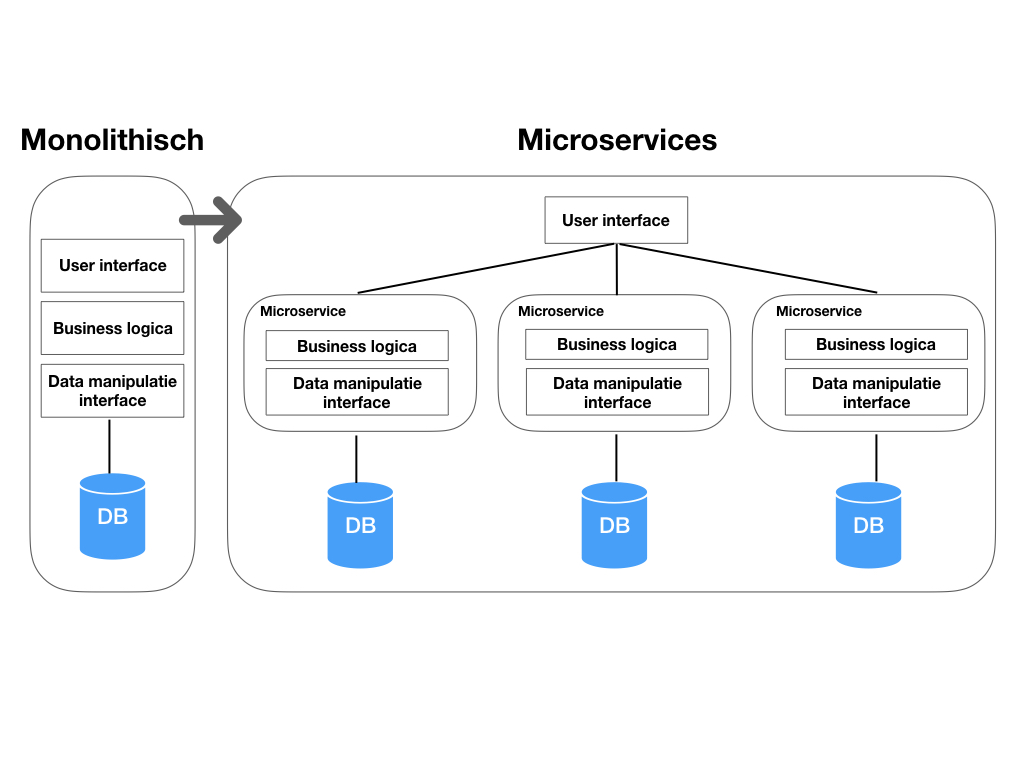
\includegraphics[width=\linewidth]{img/Microservices.jpeg}
    \caption[Monolithisch naar microservices]{High-level weergave voor migratie van monolithisch naar microservice}
    \label{fig:microservices}
\end{figure}

\section{\IfLanguageName{dutch}{Probleemstelling}{Problem Statement}}
\label{sec:probleemstelling}

% 1. Aanhalen dat Node.js er zich toe leunt om microservices te bouwen
% 2. Ik identificeer dat dit dit dit mis is bij het opbouwen van webservices in Node.js binnen een microservice-architectuur
% 3. Ik doe systematisch onderzoek naar de manieren om die dingen die vaak mis gaan goed te doen.
% 4. Wie heeft baat bij het systematisch onderzoek over de zaken die mis gaan

In dit onderzoek wordt een oplossing geformuleerd voor het consistent opbouwen van Node.js \gls{REST} services binnen een versnipperde architectuur als microservices. Er wordt geopteerd voor een TypeScript-integratie als deel van de basisopstelling, voor services meer robuust te maken en taalveiligheid voor JavaScript te garanderen.

De microservice-architectuur brengt uitdagingen met zich mee, zo wordt de business opgedeeld in verschillende onafhankelijke microservices die beheerd worden door mogelijk evenveel, of minder, autonome teams. De autonomie van elk team kan zorgen voor een verschil in technologie-stack per service, wat binnen microservices eerder een voordeel is. De technologie-stack bepaald een verzameling aan technologieën die een combinatie vormen voor het uitbouwen van de applicatie binnen een framework. \\
Het zelf bepalen van de technologie-stack geeft de vrijheid om voor services met bepaalde benodigdheden een specifiek framework te gebruiken die meer geschikt is om aan die noden te voldoen. Het bekomt echter een probleem wanneer teams onderling dezelfde technologie-stack gebruiken. 

De verdeeldheid die wordt gecreëerd onder teams, door hun autonomie binnen dezelfde organisatie, zorgt voor inconsistentie tussen services die op basis van de stack hetzelfde zouden moeten gestructureerd zijn. Het is niet mogelijk om consistentie te garanderen binnen een microservice-architectuur, op vlak van het gebruik van een bepaalde stack voor een framework, wanneer elk team hun eigen interpretatie heeft van de ``juiste'' implementatie. Het probleem is merkbaar wanneer cross-team features moeten geïmplementeerd worden door ontwikkelaars van een specifiek team of bij herstructureringen binnen de organisatie waarbij ontwikkelaars worden ingezet bij andere teams. De inconsistentie van de opstelling en structuur van de service zorgt in beide gevallen voor aanpassingsproblemen en tragere ontwikkeling.

In deze scriptie wordt systematisch onderzoek gedaan naar de juiste opbouw van \gls{REST} services in Node.js, met gebruik van de meest prominente technologieën voor het garanderen van een gefundeerde \gls{REST} \gls{API}. Dit alles voor de vrijwaring van inconsistenties onder teams die dezelfde technologie-stack gebruiken, zodat aanpassingsproblemen en ontwikkelingsvertragingen minimaal blijven in de context van cross-team features of teamherstructureringen.

\section{\IfLanguageName{dutch}{Plan van aanpak}{Overview of the approach}}
\label{sec:plan-van-aanpak}

% 1. Definieeren algemene opbouw van een Node.js webservice
% 2. De opbouw onderverdelen in verschillende fasen
% 3. Voor elk onderdeel van de websevice mogelijke technologieen aanrijken en vergelijken, waar mogelijk
% 4. De volledige webservice opbouwen met de meest gepaste technolgieen aangetoond in vorige

Het onderzoek bestaat uit 3 delen die elk instaan tot het systematisch onderzoeken van de beste opbouw voor \gls{REST} services in Node.js. Het eerste deel stelt de basisopstelling samen voor het project. Dit houdt code-linting met \emph{eslint} en \emph{prettier} in, als ook de initiatie van het project met \gls{NPM} en de configuratie voor TypeScript. \\
Daaropvolgend wordt de project-architectuur van de \gls{REST} service ontleed en wordt voor elk onderdeel, die een bepaalde technologie dient te hanteren, een vergelijkende studie gedaan tussen twee mogelijke technologieën op basis van voor- en nadelen. Hieruit wordt geconcludeerd welke de betere keuze is voor de technologie-stack en wordt op basis daarvan de implementatie in de scriptie gedocumenteerd. \\

Tot slot gebeurd een vergelijking tussen de niet gekozen technologieën en diegene die aangetoond werden beter te zijn voor de technologie-stack. De vergelijking wordt gebaseerd op tracing-statistieken voor elk project, waarbij gebruik wordt gemaakt van ``opentelemetry-js'' als open-source facilitator voor tracing. \\
Bij tracing wordt een trace gegenereerd voor processen die worden afgehandeld door de service. Zo kunnen bijvoorbeeld alle \gls{HTTP}-verzoeken gemonitord worden. Ieder sub-proces van het verzoek wordt geregistreerd zodat kan weergegeven worden uit hoeveel sub-processen het verzoek bestaat. Voor elke sub-proces, of span, wordt de executie tijd gemeten zodat een overzicht kan gemaakt worden voor de impact van een sub-proces op de gehele executie tijd van het \gls{HTTP}-verzoek.

\section{\IfLanguageName{dutch}{Opzet van deze bachelorproef}{Structure of this bachelor thesis}}
\label{sec:opzet-bachelorproef}

De rest van deze bachelorproef is als volgt opgebouwd:

% TODO: Vul hier aan voor je eigen hoofstukken, één of twee zinnen per hoofdstuk

In Hoofdstuk~\ref{ch:conclusie}, tenslotte, wordt de conclusie gegeven en een antwoord geformuleerd op de onderzoeksvragen. Daarbij wordt ook een aanzet gegeven voor toekomstig onderzoek binnen dit domein.